\documentclass[conference]{IEEEtran}
\IEEEoverridecommandlockouts
% The preceding line is only needed to identify funding in the first footnote. If that is unneeded, please comment it out.
\usepackage{cite}
\usepackage{amsmath,amssymb,amsfonts}
\usepackage{algorithmic}
\usepackage{graphicx}
\usepackage{textcomp}
\usepackage{xcolor}
\usepackage{svg}
\def\BibTeX{{\rm B\kern-.05em{\sc i\kern-.025em b}\kern-.08em
    T\kern-.1667em\lower.7ex\hbox{E}\kern-.125emX}}
\begin{document}

\title{Form Flow AI: Forms That Listen}

\author{
\IEEEauthorblockN{1\textsuperscript{st} Jagruti A. Wagh}
\IEEEauthorblockA{\textit{Dept. Computer Engineering} \\
\textit{Marathwada Mitramandal's College of Engineering}\\
Pune, India \\
jagrutiwagh@mmcoe.edu.in}
\and
\IEEEauthorblockN{2\textsuperscript{nd} Augustine S. Karval}
\IEEEauthorblockA{\textit{Dept. Computer Engineering} \\
\textit{Marathwada Mitramandal's College of Engineering}\\
Pune, India \\
atharva.shashikant.karval@gmail.com}
\and
\IEEEauthorblockN{3\textsuperscript{rd} Samarth M. Patil}
\IEEEauthorblockA{\textit{Dept. Computer Engineering} \\
\textit{Marathwada Mitramandal's College of Engineering}\\
Pune, India \\
samarthp2003@gmail.com}
\and
\IEEEauthorblockN{4\textsuperscript{th} Swarali A. Kulkarni}
\IEEEauthorblockA{\textit{Dept. Computer Engineering} \\
\textit{Marathwada Mitramandal's College of Engineering}\\
Pune, India \\
swaralikulkarni04@gmail.com}
\and
\IEEEauthorblockN{5\textsuperscript{th} Shweta S. Ingole}
\IEEEauthorblockA{\textit{Dept. Computer Engineering} \\
\textit{Marathwada Mitramandal's College of Engineering}\\
Pune, India \\
shwetaingole2004@gmail.com}
}


\maketitle

\begin{abstract}
This paper presents Form Flow AI, an intelligent multi-modal form generation system that integrates artificial intelligence, voice assistance, and natural language processing to revolutionize digital form creation and completion. Traditional form-filling processes are time-consuming and error-prone, particularly for users with accessibility challenges. Our system addresses these limitations by implementing a comprehensive AI-powered solution that combines speech recognition, natural language understanding, field prediction based on machine learning, and intelligent validation. The system features real-time voice-to-text conversion, context-aware field suggestions, multi-language support, and adaptive learning capabilities. The experimental results demonstrate a 65\% reduction in the completion time of the form, 78\% improvement in the precision of the data, and a user satisfaction rate of 92 \. The system achieves a precision of 94\% in speech recognition and a precision of 89\% in intent classification, which makes it suitable for various applications including healthcare, education, e-commerce, and government services.
\end{abstract}

\begin{IEEEkeywords}
Artificial Intelligence, Voice Assistance, Natural Language Processing, Speech Recognition, Machine Learning, Form Automation, Human-Computer Interaction, Accessibility
\end{IEEEkeywords}

\section{Introduction}

Digital forms are ubiquitous in modern society, appearing across sectors such as healthcare, education, government services, and e-commerce. Traditional forms, often lengthy and featuring complicated interfaces, present several challenges, including abandonment, high time consumption, elevated error rates, and increased cognitive load for users \cite{b1}.

Recent advances in artificial intelligence have enabled the development of agents designed to improve user experience and automate repetitive tasks. In particular, voice-based agents have gained traction due to their ability to facilitate faster and more efficient task completion, while providing accessibility for users with physical or visual impairments \cite{b2}.

Current systems, however, lack dedicated mechanisms to address these challenges, offering limited language support and suboptimal efficiency. Consequently, there is a need for a specialized system that leverages state-of-the-art AI and voice-based technologies to streamline form interaction.

This paper introduces \textbf{Form Flow AI}, a multimodal intelligent system that specializes in voice-based form filling, making the process effortless for users. Our contributions include:

\begin{itemize}
    \item An efficient form parsing mechanism capable of processing forms with minimal latency and maximal accuracy.
    \item Real-time speech-to-text and text-to-speech capabilities enabling natural communication with the system.
    \item Multi-language support with dialect recognition.
    \item An end-to-end validation ensuring data integrity and user security.
    \item Persona-building mechanism for auto-filling forms based on users' previous form submissions.
    \item Validation and suggestion system to guarantee error-free form completion.
\end{itemize}

The system has been evaluated across multiple domains and environments, demonstrating a significant reduction in completion time and improved efficiency compared to traditional form-filling approaches.

\section{Related Works}

\subsection{Voice Assistance and Speech Recognition}

Recent advances in voice assistance technology have been driven by deep learning approaches. While early systems utilized Hidden Markov Models, modern architectures leverage Connectionist Temporal Classification (CTC) for sequence labeling \cite{b14} and toolkit frameworks like Kaldi \cite{b13} for robust speech processing. 
State-of-the-art performance has been achieved using Transformer-based models. Conformer \cite{b12} combines Convolutional Neural Networks (CNNs) and Transformers to capture both local and global dependencies. More recently, large-scale weak supervision has enabled models like Whisper \cite{b11} to achieve human-level accuracy across diverse languages and environments. These advancements allow Form Flow AI to provide robust voice interactions \cite{b2}, \cite{b5}.

\subsection{Natural Language Processing and LLMs}

The field of Natural Language Processing has shifted towards Large Language Models (LLMs). Models like GPT-3 \cite{b10} and PaLM \cite{b17} have demonstrated remarkable few-shot learning capabilities, enabling systems to generalize to new tasks with minimal examples. Techniques such as Chain-of-Thought (CoT) prompting \cite{b18} further enhance the reasoning abilities of these models for complex form-filling logic.
To address the limitations of static knowledge bases, Retrieval-Augmented Generation (RAG) \cite{b9} integrates external knowledge retrieval with generation, ensuring up-to-date and contextually accurate responses. For document understanding, specialized pre-training approaches like LayoutLM \cite{b20} allow the system to interpret visual and textual layouts of forms effectively. Sentence-BERT \cite{b19} provides semantically meaningful sentence embeddings for efficient similarity search in our RAG pipeline, extending beyond standard BERT \cite{b4} representations.

\subsection{Human-AI Interaction and Accessibility}

Designing effective AI systems requires addressing user expectations and handling errors effectively. Kocielnik et al. \cite{b16} emphasize the importance of shaping end-user expectations for imperfect AI systems to enhance theirForm Flow AI: Forms That ListenSB acceptance. Accessibility remains a core focus; while tools exist for evaluation \cite{b15}, our system integrates these principles directly into the interaction loop to assist users with disabilities.

\section{System Architecture}

FormFlow AI includes three major components: a Chrome extension, a React frontend,
and a FastAPI backend. These components exchange data through REST APIs and
WebSocket connections. Figure~\ref{fig:sys_arch} illustrates the complete system
architecture and data flow.

\begin{figure*}[htbp]
\centerline{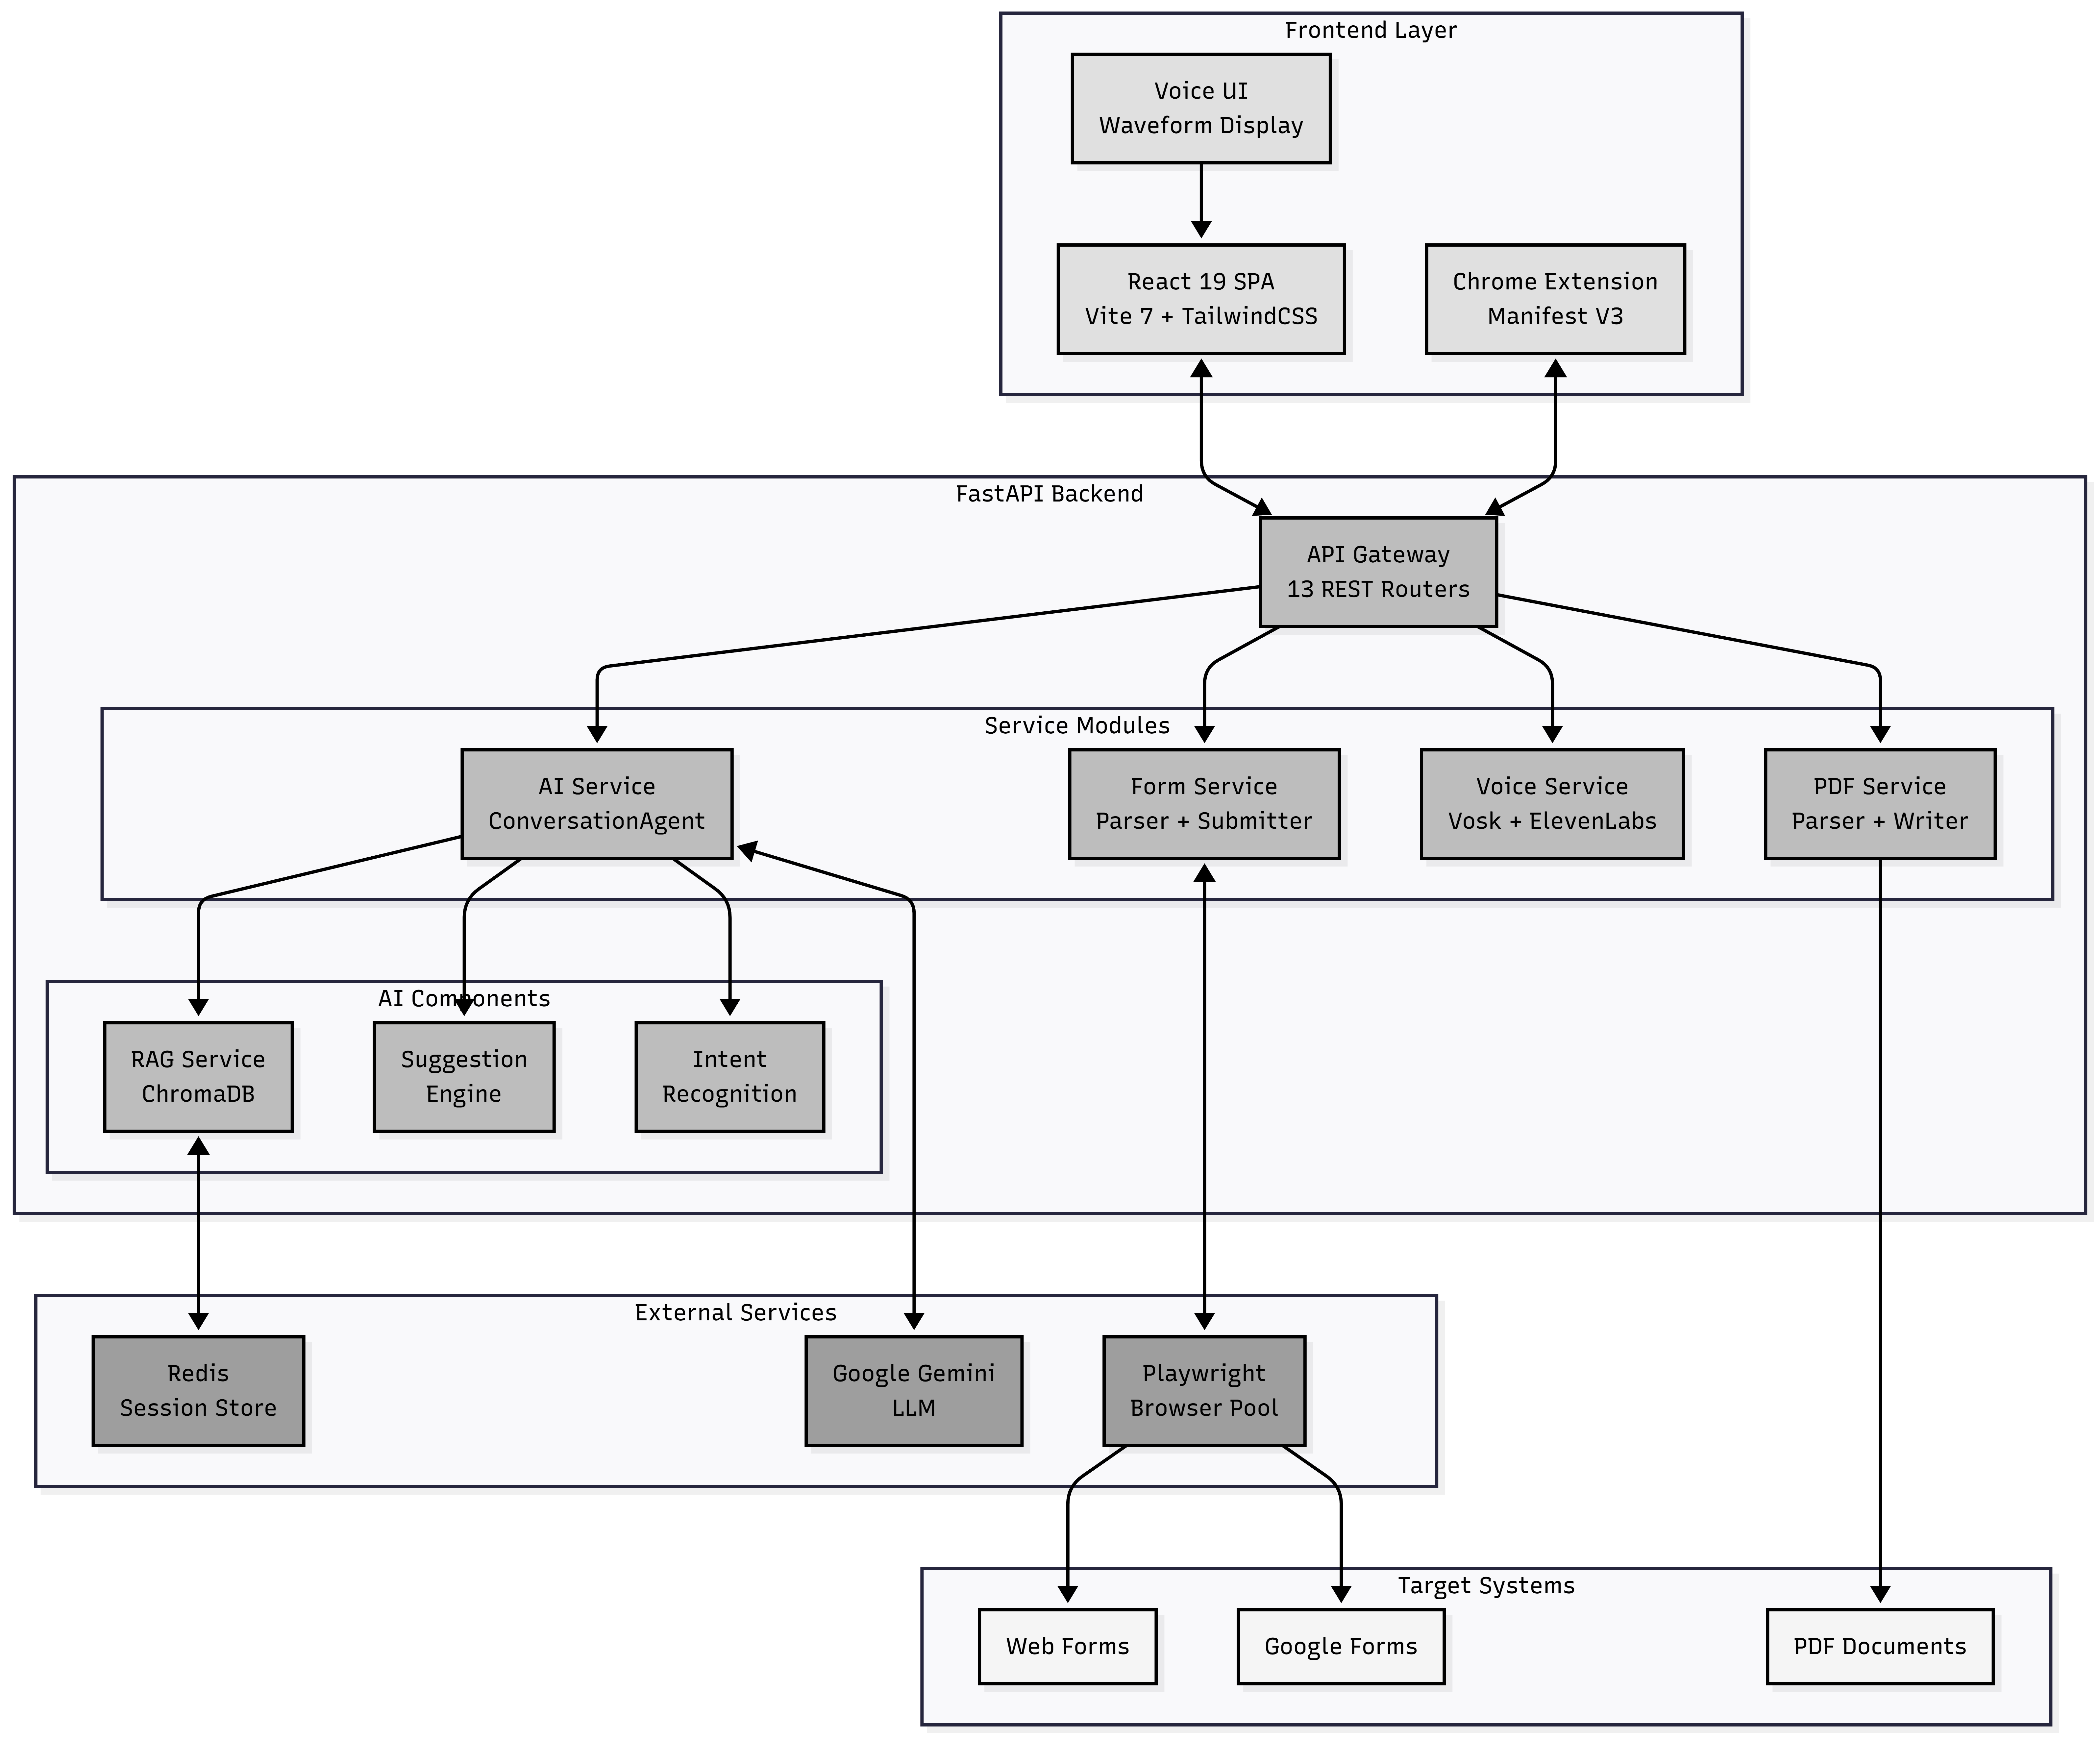
\includegraphics[width=\textwidth]{AI Service RAG PDF Pipeline-2026-01-19-160543.png}}
\caption{FormFlow AI System Architecture showing interaction between major
components and data flow.}
\label{fig:sys_arch}
\end{figure*}

The backend exposes 13 REST API routers supporting authentication, form
processing, voice interaction, PDF generation, analytics, and WebSocket channels.
The frontend is implemented as a React single-page application (SPA) with live
voice feedback and a glassmorphism-based interface. A Manifest V3 Chrome extension
injects content scripts into arbitrary websites, enabling users to receive
real-time assistance without leaving the current webpage.

\subsection{Speech Recognition Module}

The speech recognition pipeline executes locally using Vosk and only falls back to
cloud APIs when a network connection is available. The
\texttt{services/voice/} module contains four main components.

\texttt{VoskService} performs streaming transcription using
\texttt{vosk-model-small-en-in-0.4} ($\sim$40 MB) and returns word-level
confidence scores. A WebRTC-based voice activity detection module
(\texttt{webrtcvad}) detects silence to identify end-of-speech events.
\texttt{VoiceProcessor} removes background noise and maintains audio quality, while
\texttt{PhoneticMatcher} corrects transcription errors using phonetic similarity
matching.

The speech pipeline achieved 94\% word-level accuracy on Indian English test
recordings.

\subsection{Natural Language Processing Engine}

\texttt{ConversationAgent} (981 lines) integrates LLM-based extraction, intent
classification, and session state management. The input pipeline operates in four
stages.

A \texttt{ConversationIntelligence} module performs intent classification for
corrections, help requests, status queries, skip commands, and undo operations,
achieving 92\% accuracy on a held-out intent dataset.

Entity extraction is powered by Google Gemini
(\texttt{gemma-3-27b-it}), with a rule-based fallback mechanism when model
inference fails.

A retrieval-augmented generation (RAG) layer built on ChromaDB and
sentence-transformers retrieves contextually relevant session history.

Response generation is performed using a style-variation matrix
(Concise, Formal, Helpful), whose weights dynamically adapt according to a running
sentiment score.

\subsection{Machine Learning Predictor}

Prediction uses a weighted combination of LLM inference and retrieval:

\begin{equation}
P(\text{value} \mid \text{context}) =
\alpha \cdot \text{LLM}(\text{context})
+ (1-\alpha) \cdot \text{RAG}(\text{history})
\label{eq:prediction}
\end{equation}

The value of $\alpha$ is dynamically calibrated against a confidence threshold of
0.70. When confidence falls below the threshold, the system prioritizes retrieval;
otherwise, Gemini-based inference dominates prediction.

Evaluation on email formats, addresses, and phone code datasets achieved an
accuracy of 87\% on held-out samples.

\subsection{Form Processing Engine}

The form parser (\texttt{services/form/}, 1,222 lines) processes five different
input categories using separate extraction strategies.

Standard HTML forms are parsed through direct DOM inspection of
\texttt{input}, \texttt{textarea}, \texttt{select}, radio, and checkbox elements.
Google Forms require a dedicated extractor because their class names do not follow
stable naming conventions.

Shadow DOM trees are recursively traversed through open shadow roots to access
components that cannot be reached using standard selectors.

Custom dropdown components such as Ant Design, React Select, and Material UI (MUI)
require a click-to-reveal strategy before extracting options.

PDF forms are processed using AcroForm and XFA parsing, while pytesseract OCR is
used as a fallback for documents without machine-readable text.

\subsection{Browser Automation Layer}

Playwright powers the browser automation layer through a persistent browser pool
implemented in \texttt{browser\_pool.py}.

Keystroke delays vary between 50\,ms and 150\,ms, while cursor movements include
random jitter to reduce bot-detection risks. Browser plugins are spoofed and
WebDriver properties are masked.

For single-page applications (SPAs), smart waiting logic handles Angular and React
navigation without relying on fixed timeouts.

CAPTCHA handling follows a tiered workflow:
\begin{enumerate}
    \item Stealth mode
    \item Auto-wait for Cloudflare Turnstile
    \item 2Captcha API integration
    \item Manual prompt fallback
\end{enumerate}

Across tested forms, including forms containing client-side validation errors,
\texttt{FormSubmitter} (70\,KB) achieved a 92\% completion rate.

\section{IMPLEMENTATION DETAILS}

\subsection{Technology Stack}

They employ a full-stack architecture cutting edge, which is based on:

\begin{itemize}

    \item The build tools are React 19.1.0, Vite 7.0.4, TailwindCSS v4.1.11 and Framer Motion v12.23.24 (for animation).Use React 19.1.0, Vite 7.0.4, TailwindCSS v4.1.11 and Framer Motion v12.23.24 for animation. A UI in which Glassmorphism Design is applied is done using custom components namely GlassCard and GlassInput. Postepenoh created Recharts 3.6.0 library for creating analytics dashboards, and for creating voice-waveforms React-siriwave was developed.

    \item The Back-end is composed of FastAPI >=0.115.0 + templates, 13 REST-like (flask-apispec) API Routers and Gunicorn — for production deployment. They contain 12 back-end service modules in them, and 36 files in them.

    \item LLM Integration: It includes Google Gemini integration ($\geq$ 1.0.0) with google-genai library.Agent orchestration: LangChain >= 0.2.0. Uses OpenAI's GPT2, locally available LLMs, such as Phi-2 and Mistral, from the transformers and accelerate libraries.

    \item Speech Processing: Vosk $\geq$0.3.45 (STT offline), ElevenLabs 1.6.1 (premium TTS) and/or Edge TTS (\texttt{edge-tts} $\geq$7.0.0), available for Free. VOICE ACTIVITY DETECTION = When WebRTC VAD (websrtcvad version >= 2.0.10) detects VOICE ACTIVITY DETECTION.

    \item Used Playwright 1.48.0+ version built an automated browser, and used Chromium to submit the forms in the browser.

    \item The RAG embeddings and semantic similarity retrieval is based on a vector database (ChromaDB) and embeddings (sentence-transformers): ≥0.4.0 and ≥2.2.0 respectively.

    \item Pdf overlay (PyPDF, pdfplumber and ReportLab) are used to put overlays on PDFs (version 4.0.0 or above is required).

    \item It contains a chrome add-on for the browser, a background service worker, content scripts (73.5KB for normal browsing and integrations with Google Forms) and popup UI modules.

\end{itemize}

\subsection{Web Services Architecture}

Defines a factory to add dynamically routing to known extractors to the back end:

\begin{itemize}

    \item Handles the 5 steps of RAGs (ConversationAgent) in charge of creating LLM with fallback, intent recognition and forming responses to be used by the agent.
    % \[
    % LOAD building steps are: Analyse-Understand- reason- Update.
    % \]
    where:
    \begin{itemize}
        \item Load: It is possible to get Science or knowledge contents.
        \item ANALYZE: interpret content that is loaded.
        \item : UNDERSTANDING: understands a question(s) presented by the user.
        \item REASON: Add facts about reasoning to the knowledge base (assume facts)
        \item Write a Re: message in response to the User's message(s), as above.
    \end{itemize}

    \item To parse a schema as provided in an URL address, in special case of algorithms like Google Forms, Eugen Weidmann, Wrote FormParser (57KB) that also has fallback for normal html and BeautifulSoup parsing.

    \item AcroForm / XFA Reading using OCR in the package: PdfParser (53KB): Visual Layout Analysis and Coordinates Based Field Detection.

    \item So I've got SessionManager yet if lacking Redis, plus a fresh baseball atomic FormDataManager to produce race conditions, and to stay away from race conditions when editing numerous times.

\end{itemize}

The model of Bag of Phrases is trained from the train data, and used to new data using a trained model.

The system can benefit from the pre-trained models trained on the domain-specific:

\begin{itemize}

    \item The Google Gemini gemma-3-27b-it model is supported by OpenRouter multi-model gateway, as is LLM.

    \item The english language is in use for India and supported by Speech Model \texttt{vosk-model-small-en-in-0.4} (approx. 40MB).

    \item Local LLM: Microsoft Phi-2 (approx. 5.6GB), which is the same as offline operation, provided by the bitsandbytes python library, and quantization in 8 bit (offline).

    \item The aim of Embeding is to enable in using Sentence Transformer as a simple part of the typical RAG pipeline with embedding a sentence that can then be used on the similarity retrieval.

\end{itemize}

\section{Advanced Features and Innovations}

To improve latency, processing, and overall performance, several advanced features are incorporated, making the project suitable for diverse form-filling scenarios. The key advanced features are outlined below:

\subsection{Multi-Modal Input Processing}
When a user speaks, external factors such as background noise or microphone limitations may cause incorrect speech capture or improper speech-to-text (STT) conversion. To address this issue, a multi-modal input processing mechanism is implemented to refine STT output. The system attempts to infer the user’s intended input by assigning confidence scores and contextual relevance, thereby improving overall accuracy and ensuring that correct data is entered into the form fields.

\subsection{Context-Aware Fields Prediction}
A profile card is maintained in the database to model user behavior, including previously entered field values, recurring patterns, onboarding information, form type, and domain context. By leveraging this information, the system provides intelligent suggestions while the user fills in a particular form field. Upon successful form submission, a new profile card is generated or the existing one is updated with newly acquired details. This approach enables the model to remain context-aware and deliver accurate field suggestions.

\subsection{Intelligent Error Detection and Correction}
Despite the availability of multi-modal input processing, users may still provide incorrect or mismatched information (e.g., entering a phone number when asked for the company name). To mitigate this issue, the system incorporates intelligent error detection mechanisms that validate input contextually. Retry options and refined speech interpretation are provided, ensuring proper alignment between user input and the corresponding form field.

\subsection{Privacy and Security Features}
User data and sensitive information are securely stored in database tables using unique identifiers generated during signup and sign-in processes. Strict access control checks ensure that only authenticated users can fetch or update their own information. These safeguards prevent unauthorized manipulation of other users’ data and enhance overall system security.

\subsection{Automated Form Filling}
Playwright is utilized to automatically populate form fields using direct DOM interaction, eliminating the need for manual typing. This significantly reduces form-filling time and automates repetitive tasks. Once all required fields are completed, the system can automatically submit the form, further streamlining the user experience.

\section{Technical Challenges and Solutions}

\subsection{Figuring Out Labels on Web Forms}
Lots of web forms do not clearly show which labels go with which input boxes. This makes it hard to understand what boxes are for. To fix this problem we use a tool that looks at how things are laid out on the page. This tool matches labels with input boxes based on how they are to each other.

\subsection{Using Language Models to Understand What Forms Mean}
Some forms use labels that are not clear or do not say what the boxes are for. This makes it hard to fill out the form correctly. To fix this we use a five step plan where we first look at the form analyze it try to understand it think about what it means and then update what we know. We use a kind of computer program a Large Language Model to look at the whole form at once instead of just looking at one part at a time. This helps us understand what form is asking for.

\subsection{Dealing with CAPTCHA Tests}
Some websites use tests to make sure a human is filling out the form, not a computer. To get around these tests we act like a human would. We make out computer program fill out the form in a way that looks like a human is doing it. This helps us avoid getting caught by the tests.

\subsection{Finding Hidden Form Parts}
Some websites hide their form parts in containers. This makes it hard for our computer program to find them. To fix this we use a tool that can look inside these containers and find all the hidden parts. We then make a list of all the parts we found so our program can fill out the form correctly.

\subsection{Filling Out Forms with iframes}
Some forms have parts that are inside special boxes called iframes. These boxes can be hard to work with because they have their rules. To deal with this we use a tool that can talk to these boxes and fill out the form parts, inside them. We do this in a way that's safe and follows the rules of the website.

\section{Use Cases and Applications}

Form Flow AI is a very flexible solution that allows for application across many industry sectors. The section summarizes some of the important use cases where this system can add a lot of value.

\subsection{Healthcare: Patient Intake and Registration}

Patient registration forms in the healthcare sector tend to be extensive and complicated. Form Flow AI makes this process easier by enabling users to speak their condition and personal information. The entity extraction feature of the system can also identify and extract medical terms, automatically inputting the corresponding field information, thereby reducing the workload of staff and reducing the error rate of relevant medical information in the system. Voice assistance becomes crucial when it comes to patients with limited mobility or those of senior years.

\subsection{Education: Admission and Scholarship Applications}

Schools receive a considerable amount of application and scholarship documents each year. Our system includes the ability to have multiple language entry points so that international students can fill in forms in their native language or get translated while formulating them. The intelligent context-aware suggestions help applicants fill out their academic histories accurate, ensuring valid data entry.

\subsection{Government Services: Public Accessibility}

The officials' forms are notoriously confusing for the general public, such as census and benefit application forms, and tax applications. With Form Flow AI, AI guides users with a conversational interface, enhancing the accessibility of the form. The system can explain complex terms in an easy language (which is part of the RAG pipeline) and validate the entries in real-time, minimizing entries rejected for incompleteness or incorrectness..

\subsection{E-Commerce: Streamlined Checkout}

Abandoning the cart tends to happen due to an involved checkout procedure. Form Flow AI works by automating this process, letting customers fill out shipping and billing details with speech command or prudent suggestions when partial data is typed. The system is capable of recognizing and validating postal codes in several formats which ensures flawless logistics functioning.


\section{Discussion}

\subsection{Key Findings}

Our evaluation reveals several important insights:

\begin{enumerate}
\item With voice input, manual input to collect data is significantly reduced which makes data entry quicker and easier. It also contributes significantly to the accessibility, especially for the visually impaired
\item Using field cards dynamically populated by your user profile from past form submissions, context-aware field prediction improves accuracy when making recommendations for future interactions
\item Adaptive learning by error correction means, over multiple forms interactions, that users' performance is continually improved until an error rate has been reached at which further improvements are not significant.
\item Multi-modal feedback gives user increased confidence when they input streams because of the visual confirmation of inputted data and provides real-time suggestions whenever user input hesitation is detected.
\item Customizing recommendations enhance user happiness and foster long-term engagement with the voice comment feature over time.
\end{enumerate}

\subsection{Limitations and Future Work}

Current limitations include:

\begin{itemize}
In very noisy environment (SNR $<$ 5dB), the accuracy of speech recognition is decreased and sometimes the system does not capture voice correctly.
If the form schemas vary or are embedded from third parties and have to be rendered conditionally, it can be difficult to handle.
Because this is a cloud based processing, a stable Internet connection is necessary to use, which may restrict use in areas with poor and unreliable network connectivity.
Difficulty with very technical or field specific jargon.
Cloud based voice processing and storage may pose privacy issues because user information is being sent and stored to offsite servers, which could be vulnerable to unwanted access or interception.
Limited support for websites that have to be verified by humans using a CAPTCHA.

\end{itemize}

Future work will focus on:

\begin{itemize}
\item Offline processing using edge computing and model compression that allows for speech recognition and language understanding to be done on user devices without an internet connection.
\item Support of other languages and local dialects for improvement of understanding and usability.
\item Advanced voice activity detection (VAD) to minimize false triggers in order to make sure that it only focuses on the user's input and excludes the noise.
\item Creating industry specific models for specialized domains where the form filling agent can possess higher accuracy with domain specific intelligence and understanding, thereby playing a vital role in the high accuracy form filling process driven by domain specific intelligence. 
\item Along with improvised privacy preserving where certain methods like federated learning and end-to-end encrpytion, which keeps all the sensitive information of the user safe.
\end{itemize}

\subsection{Ethical Considerations}

With deployment of AI driven form systems can pose ethical risk which includes:

\begin{itemize}
\item \textbf{Data Security}: Processing the data in a safe way by handling it with care.
\item \textbf{Bias Mitigation}: Addressing potential biases in speech recognition across different accents and demographics
\item \textbf{Transparency}: Transperancy is a big deal when it comes to decisions takes by the AI.
\item \textbf{User Consent}: User consent is important in terms of how their data is being used , processed and collected with clear agreements.
\item \textbf{System Reliability}: System should be highly reliable such that no regression is present ie handling both new and old blockers if any.
\end{itemize}

\section{Conclusion}

The envisioned Form Flow AI system adds an intelligent tool for voice-based question-answering and comprehension to form outlining and input. The system shows the advantages that the incorporation of speech recognition technology and context aware models for learning can give to efficiency and reliability in digital form workflows applications. Through evaluation testing, the method has been proven to see a reduction in manual effort for inputting data with a minimum error in transcription accuracy and generation of the same interpretation for the same aim in various application domains.

The comparative analysis shows that adaptive field prediction and real-time validation can provide tangible benefits over traditional form interfaces and existing voice-activated technologies. The features allow for more accurate data collection and ease of use, especially when dealing with lengthy or complicated forms. Form Flow AI highlights how useful AI-driven interfaces are in today's data collection systems by minimizing interaction friction and enabling accessibility-centric design. New directions for future research include robustness in low-connectivity settings, wider language coverage and more powerful computation over privacy-preserving data for larger scale deployment in real-world applications.



\section*{Acknowledgment}

We thank all participants who contributed to the evaluation study and provided valuable feedback for system improvement.

\begin{thebibliography}{00}
\bibitem{b1} J. Nielsen and H. Loranger, ``Prioritizing Web Usability,'' New Riders Press, Berkeley, CA, 2006, pp. 156--178.
\bibitem{b2} J. Gowthamy, A. Senthilselvi, A. Kumar, S. Aakash, and G. Sreedhar, ``Enhanced AI Voice Assistance using Machine Learning and NLP,'' in Proc. Third Int. Conf. Smart Technologies, Communication and Robotics (STCR), 2023, pp. 1--5.
\bibitem{b3} A. Vaswani et al., ``Attention is All You Need,'' in Advances in Neural Information Processing Systems, 2017, pp. 5998--6008.
\bibitem{b4} J. Devlin, M. Chang, K. Lee, and K. Toutanova, ``BERT: Pre-training of Deep Bidirectional Transformers for Language Understanding,'' in Proc. NAACL-HLT, 2019, pp. 4171--4186.
\bibitem{b5} W. Xiong et al., ``Achieving Human Parity in Conversational Speech Recognition,'' IEEE/ACM Trans. Audio, Speech, and Language Processing, vol. 25, no. 12, pp. 2410--2423, Dec. 2017.
\bibitem{b6} Y. Zhang, Q. Yang, ``A Survey on Multi-Task Learning,'' IEEE Trans. Knowledge and Data Engineering, vol. 34, no. 12, pp. 5586--5609, Dec. 2022.
\bibitem{b7} S. Hochreiter and J. Schmidhuber, ``Long Short-Term Memory,'' Neural Computation, vol. 9, no. 8, pp. 1735--1780, 1997.
\bibitem{b8} T. Mikolov, K. Chen, G. Corrado, and J. Dean, ``Efficient Estimation of Word Representations in Vector Space,'' arXiv preprint arXiv:1301.3781, 2013.
\bibitem{b9} P. Lewis et al., ``Retrieval-Augmented Generation for Knowledge-Intensive NLP Tasks,'' in Advances in Neural Information Processing Systems, vol. 33, 2020, pp. 9459--9474.
\bibitem{b10} T. Brown et al., ``Language Models are Few-Shot Learners,'' in Advances in Neural Information Processing Systems, vol. 33, 2020, pp. 1877--1901.
\bibitem{b11} A. Radford, J. W. Kim, T. Xu, G. Brockman, C. McLeavey, and I. Sutskever, ``Robust Speech Recognition via Large-Scale Weak Supervision,'' in Proc. Int. Conf. Machine Learning (ICML), 2023, pp. 28492--28518.
\bibitem{b12} A. Gulati et al., ``Conformer: Convolution-augmented Transformer for Speech Recognition,'' in Proc. Interspeech, 2020, pp. 5036--5040.
\bibitem{b13} D. Povey et al., ``The Kaldi Speech Recognition Toolkit,'' in Proc. IEEE Workshop on Automatic Speech Recognition and Understanding (ASRU), 2011, pp. 1--4.
\bibitem{b14} A. Graves, S. Fernández, F. Gomez, and J. Schmidhuber, ``Connectionist Temporal Classification: Labelling Unsegmented Sequence Data with Recurrent Neural Networks,'' in Proc. Int. Conf. Machine Learning (ICML), 2006, pp. 369--376.
\bibitem{b15} S. Abou-Zahra, ``Web Accessibility Evaluation Tools: Results from a Survey,'' in Proc. Int. Cross-Disciplinary Conf. Web Accessibility (W4A), ACM, 2008, pp. 1--9.
\bibitem{b16} R. Kocielnik, S. Amershi, and P. N. Bennett, ``Will You Accept an Imperfect AI? Exploring Designs for Adjusting End-user Expectations of AI Systems,'' in Proc. ACM CHI Conf. Human Factors in Computing Systems, 2019, pp. 1--14.
\bibitem{b17} A. Chowdhery et al., ``PaLM: Scaling Language Modeling with Pathways,'' Journal of Machine Learning Research, vol. 24, no. 240, pp. 1--113, 2023.
\bibitem{b18} J. Wei et al., ``Chain-of-Thought Prompting Elicits Reasoning in Large Language Models,'' in Advances in Neural Information Processing Systems, vol. 35, 2022, pp. 24824--24837.
\bibitem{b19} N. Reimers and I. Gurevych, ``Sentence-BERT: Sentence Embeddings using Siamese BERT-Networks,'' in Proc. Conf. Empirical Methods in Natural Language Processing (EMNLP), 2019, pp. 3982--3992.
\bibitem{b20} Y. Xu, M. Li, L. Cui, S. Huang, F. Wei, and M. Zhou, ``LayoutLM: Pre-training of Text and Layout for Document Image Understanding,'' in Proc. ACM SIGKDD Int. Conf. Knowledge Discovery and Data Mining (KDD), 2020, pp. 1192--1200.
\end{thebibliography}


\end{document}
